\documentclass{beamer}

\usepackage{amsmath}
\usepackage{amsfonts}
\usepackage{amssymb}
\usepackage{listings}
\usepackage{graphicx}
\usepackage{tikz}

\graphicspath{{../}}

% KCPC theme
\usetheme{default}
\useinnertheme{rectangles}
\useoutertheme{default}

\beamerdefaultoverlayspecification{<+->}

\setbeamertemplate{navigation symbols}{}

% Colours
\definecolor{kcpc-bg}{RGB}{250,250,250}
\definecolor{kcpc-text}{RGB}{20,20,20}
\definecolor{kcpc-muted}{RGB}{90,90,90}
\definecolor{kcpc-red}{RGB}{176,0,0}

\setbeamercolor{background canvas}{bg=kcpc-bg}
\setbeamercolor{normal text}{fg=kcpc-text}
\setbeamercolor{frametitle}{fg=kcpc-text,bg=kcpc-bg}
\setbeamercolor{title}{fg=kcpc-text}
\setbeamercolor{subtitle}{fg=kcpc-muted}
\setbeamercolor{structure}{fg=kcpc-red}

\setbeamerfont{title}{series=\bfseries,size=\Large}
\setbeamerfont{frametitle}{series=\bfseries,size=\large}

\setlength{\parskip}{0.4em}

\setbeamertemplate{itemize item}{$\rightarrow$}
\setbeamertemplate{itemize subitem}{$\rightarrow$}

\setbeamertemplate{headline}{
    \vspace{0.2cm}
    \hspace{0.2cm}
    \textcolor{kcpc-muted}{\small\insertsection}
    \hfill
}

\setbeamertemplate{footline}{
    \hspace{0.2cm}
    \textcolor{kcpc-muted}{\small KCPC}
    \hfill
    \vspace{0.3cm}
}

\setbeamertemplate{background}{
    \begin{tikzpicture}[remember picture,overlay]
        \node[
            opacity=0.035,
            at=(current page.center)
        ] {
            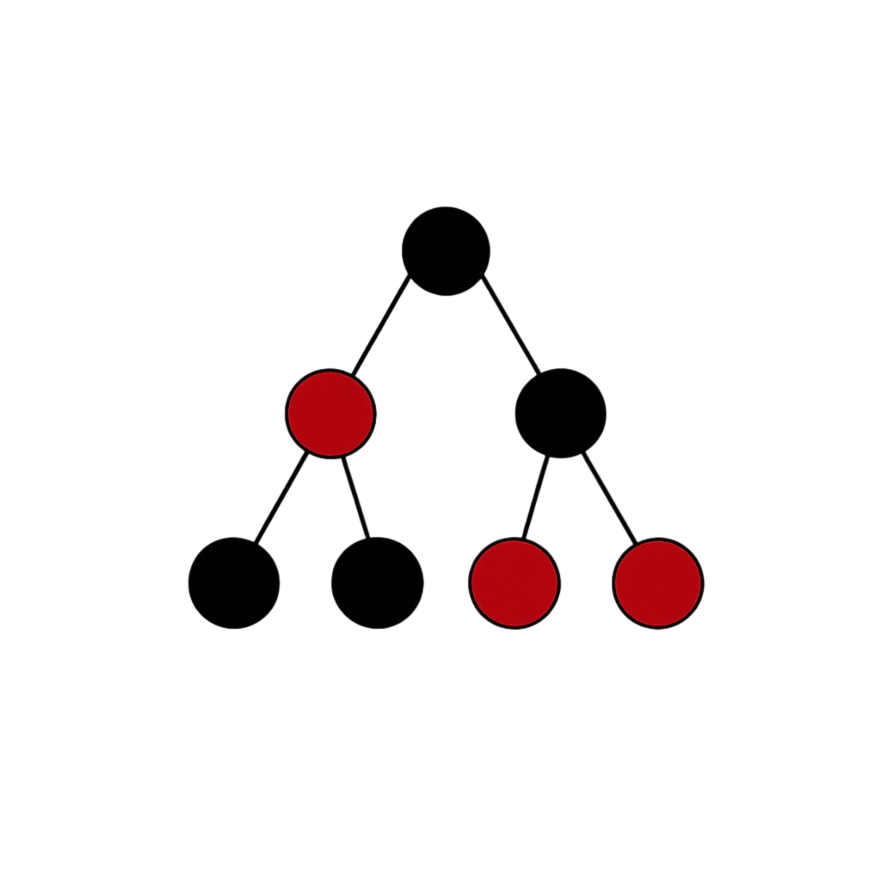
\includegraphics[width=0.55\paperwidth]{kcpc-logo.png}
        };
    \end{tikzpicture}
}

\AtBeginSection[]{
    \begin{frame}[plain]
        \vfill
        \centering
        {\Large\bfseries \insertsection}
        \vfill
    \end{frame}
}

\title{Mathematical Problem Solving I}
\subtitle{Logic, Invariants, Colouring and Induction}
\author{KCPC}
\date{Week 1}

\begin{document}

\begin{frame}
    \titlepage
\end{frame}

\begin{frame}{Overview}
    \tableofcontents
\end{frame}

\section{Competitive Programming}

\begin{frame}{What Is Competitive Programming?}
    \pause
    \begin{itemize}
        \item Competitive programming is a sport about solving problems
            with algorithms.
        \item You are given a problem statement, input, output, and constraints.
        \item You design an algorithm that always gives the right answer.
        \item You implement it in code and submit it to an automatic judge.
        \item The judge checks your program on many hidden test cases.
        \item The challenge is not just solving it once. It is solving
            every valid case quickly enough.
    \end{itemize}
\end{frame}

\begin{frame}{Why Start With Mathematical Puzzles?}
    \pause
    \begin{itemize}
        \item Many CP problems are puzzles wearing programming clothes.
        \item The computer will not rescue a bad idea. It will just
            run it faster.
        \item We want to practise spotting structure before worrying
            about syntax.
        \item Today is about the thinking tools behind many
            algorithmic solutions.
        \item Once the idea is clear, implementation becomes much
            less mysterious.
    \end{itemize}
\end{frame}

\begin{frame}{What Do You Need To Start?}
    \pause
    \begin{itemize}
        \item Do not worry: GCSE/A-level maths is enough to get started.
        \item No secret theorem is required. All you need is some
            patience and willingness to have a go.
        \item The goal is not to be fast. It is to notice what is
            really going on.
        \item A good solution should feel less like a trick, and more
            like finally seeing the shape of the problem.
        \item If you already have a stronger foundation, we have left
            some harder questions for you to tackle.
    \end{itemize}
\end{frame}

\section{Logic}

\begin{frame}{What is Logic?}
    \pause
    \begin{itemize}
        \item Logic is the study of \textbf{reasoning}:
            how conclusions follow from assumptions or available information.
        \item It helps us distinguish between:
            \begin{itemize}
                \item what is \textbf{true or false} in the world;
                \item what each person can \textbf{observe};
                \item what each person \textbf{knows} from those observations;
                \item what each person knows about \textbf{what others know};
                \item what people can \textbf{infer} from each other's actions,
                    statements, or information;
                \item what \textbf{silence, inaction, or missing information}
                    can reveal.
            \end{itemize}
        \item A central question is:
            \begin{center}
                \emph{``Given what I know, and what I know about what
                    others know,
                what must be true?''}
            \end{center}
    \end{itemize}
\end{frame}

\begin{frame}{Worked Example: Two Doors}
    You face two doors. One leads out; one does not.

    One guard always tells the truth. The other always lies. You do not
    know which guard is which.

    \vspace{0.5em}
    You may ask one guard one yes/no question. How do you find the safe door?
\end{frame}

\begin{frame}{Solution: Two Doors}
    \pause
    \begin{itemize}
        \item Ask either guard: ``Would the other guard say this door is safe?''
        \item If you asked the truth-teller, they truthfully report the
            liar's false answer.
        \item If you asked the liar, they lie about the truth-teller's
            correct answer.
        \item Either way, the answer points to the unsafe door. Choose
            the other one.
    \end{itemize}
\end{frame}

\begin{frame}{Student Exercises}
    \begin{itemize}
        \item<1-> Basic: Same Birthday Month.
        \item<1-> Easy: Glove Selection.
        \item<1-> Medium: Two Doors.
        \item<1-> Hard: Islander Statements.
        \item<1-> Very Hard: Counterfeit Coin.
    \end{itemize}
\end{frame}

\section{Invariants}

\begin{frame}{What is an Invariants?}
    \pause
    \textbf{An invariant} is a quantity or property that stays
    unchanged after every legal move.

    Invariants are useful because they can show that a certain position
    is impossible to reach without checking every possible sequence of moves.

    Common invariants include:
    \pause
    \begin{itemize}
        \item parity: odd or even;
        \item divisibility or remainder modulo $m$;
        \item number of connected components;
        \item colour balance;
        \item XOR or binary properties.
    \end{itemize}
\end{frame}

\begin{frame}{Worked Example: Last Ball}
    A bag contains black and white balls.

    Repeatedly remove two balls:
    \begin{itemize}
        \item<1-> same colours: put back one black ball;
        \item<1-> different colours: put back one white ball.
    \end{itemize}

    Can we predict the colour of the last ball?
\end{frame}

\begin{frame}{Solution: Last Ball}
    \pause
    \begin{itemize}
        \item Track the parity of the number of white balls.
        \item Removing two black balls: white parity unchanged.
        \item Removing two white balls and adding black: white count
            changes by $-2$.
        \item Removing one of each and adding white: white count unchanged.
        \item The parity of the number of white balls is invariant.
        \item The last ball is white if the initial white count was odd,
            and black if it was even.
    \end{itemize}

\end{frame}

\begin{frame}{Student Exercises}
    \begin{itemize}
        \item<1-> Basic: Jigsaw Assembly.
        \item<1-> Easy: Odd Handshakes.
        \item<1-> Medium: Chameleons.
        \item<1-> Hard: MU Puzzle.
        \item<1-> Very Hard: Fifteen Puzzle.
    \end{itemize}
\end{frame}

\section{Colouring Arguments}

\begin{frame}{What are Colouring Arguments?}
    \pause
    A \textbf{colouring argument} assigns colours to parts of a
    problem so that a hidden pattern becomes easier to see.

    It is useful when moves, paths, or tiles interact with the
    colours in a predictable way.

    Colouring arguments turn a geometric problem into a counting or
    parity problem.

    Examples:
    \pause
    \begin{itemize}
        \item a domino covers one black and one white square;
        \item a knight always moves to a square of the opposite colour;
        \item a path through adjacent grid squares alternates between colours.
    \end{itemize}

\end{frame}

\begin{frame}{Worked Example: Deficient Chessboard}
    Remove two diagonally opposite corners from a chessboard.

    Can the remaining board be tiled by $31$ dominoes?
\end{frame}

\begin{frame}{Solution: Deficient Chessboard}
    \pause
    \begin{itemize}
        \item Colour the board as a chessboard.
        \item Opposite corners have the same colour.
        \item Removing them leaves $32$ squares of one colour and
            $30$ of the other.
        \item Every domino covers exactly one of each colour.
        \item A tiling would need equal colour counts, so it is impossible.
    \end{itemize}
\end{frame}

\begin{frame}{Student Exercises: Colouring}
    \begin{itemize}
        \item<1-> Basic: One Missing Corner.
        \item<1-> Easy: Corner-To-Corner Knight Journey.
        \item<1-> Medium: Board Walks.
        \item<1-> Hard: Jumping To The Other Side.
        \item<1-> Very Hard: Domino Tiling Revisited.
    \end{itemize}
\end{frame}

\section{Induction and Monovariants}

\begin{frame}{What is Induction?}
    \pause
    \textbf{Induction} is a method for proving that a
    statement is true for every positive integer.

    The idea is that once the first case is true, each case forces
    the next one to be true.

    Induction is useful when a problem of size $n+1$ can be related
    to the same problem of size $n$.

    It typically goes like this:
    \pause
    \begin{itemize}
        \item \textbf{Base case:} prove the statement is true for the
            smallest value, usually $n=1$.
        \item \textbf{Induction step:} assume the statement is true
            for some $n$, and use this to prove it is true for $n+1$.
    \end{itemize}
\end{frame}

\begin{frame}{Monovariants}
    \pause
    A \textbf{monovariant} is a quantity that always moves in one
    direction, such as always decreasing or always increasing.

    It is useful for proving termination or impossibility.

    What to look out for:
    \pause
    \begin{itemize}
        \item total number of pieces increases;
        \item distance to a target decreases;
        \item perimeter never increases;
        \item number of bad pairs decreases.
    \end{itemize}
\end{frame}

\begin{frame}{Worked Example: Chocolate Bar}
    An $n\times m$ chocolate bar must be broken into unit squares.

    Each move breaks exactly one existing piece in a straight line.

    What is the minimum number of breaks?
\end{frame}

\begin{frame}{Solution: Chocolate Bar}
    \pause
    \begin{itemize}
        \item Track progress instead of the shape of the pieces.
        \item The final bar has $nm$ unit pieces.
        \item Each break increases the number of pieces by exactly 1.
        \item Starting from 1 piece, reaching $nm$ pieces needs
            $nm-1$ increases.
        \item Therefore every successful method uses exactly $nm-1$ breaks.
    \end{itemize}
\end{frame}

\begin{frame}{Student Exercises: Induction and Monovariants}
    \begin{itemize}
        \item<1-> Basic: Breaking A Chocolate Bar.
        \item<1-> Easy: Induction Inequality $n!>2^n$.
        \item<1-> Medium: Infected Chessboard.
        \item<1-> Hard: Parliament Pacification.
        \item<1-> Very Hard: Pebble Spreading.
    \end{itemize}
\end{frame}

\begin{frame}{Wrap-Up}
    \pause
    \begin{itemize}
        \item \textbf{Logic} tracks \textbf{knowledge} and what can be inferred.
        \item \textbf{Invariants} track what \textbf{cannot change}.
        \item \textbf{Colouring} turns \textbf{geometry into counting}.
        \item \textbf{Induction} reduces a problem to a \textbf{smaller case}.
        \item \textbf{Monovariants} track \textbf{progress} and can
            reveal \textbf{impossibility}.
    \end{itemize}
\end{frame}

\begin{frame}{What's more?}
    \pause
    \begin{itemize}
        \item Wishful thinking: simplify the problem.
        \item Symmetry: pair, reflect, and cancel.
        \item Extreme principle: look at the largest, smallest, or
            boundary case.
        \item Reduction: change the representation or reduce to a
            familiar problem.
    \end{itemize}
\end{frame}

\begin{frame}{Thanks for coming!}
    \begin{center}
        \Large
        \textbf{See ya next week!}

        I hope you enjoyed the workshop and found some useful new
        ways to approach problems.
    \end{center}
\end{frame}

\end{document}
